% Options for packages loaded elsewhere
% Options for packages loaded elsewhere
\PassOptionsToPackage{unicode}{hyperref}
\PassOptionsToPackage{hyphens}{url}
\PassOptionsToPackage{dvipsnames,svgnames,x11names}{xcolor}
%
\documentclass[
  letterpaper,
  DIV=11,
  numbers=noendperiod]{scrartcl}
\usepackage{xcolor}
\usepackage{amsmath,amssymb}
\setcounter{secnumdepth}{-\maxdimen} % remove section numbering
\usepackage{iftex}
\ifPDFTeX
  \usepackage[T1]{fontenc}
  \usepackage[utf8]{inputenc}
  \usepackage{textcomp} % provide euro and other symbols
\else % if luatex or xetex
  \usepackage{unicode-math} % this also loads fontspec
  \defaultfontfeatures{Scale=MatchLowercase}
  \defaultfontfeatures[\rmfamily]{Ligatures=TeX,Scale=1}
\fi
\usepackage{lmodern}
\ifPDFTeX\else
  % xetex/luatex font selection
\fi
% Use upquote if available, for straight quotes in verbatim environments
\IfFileExists{upquote.sty}{\usepackage{upquote}}{}
\IfFileExists{microtype.sty}{% use microtype if available
  \usepackage[]{microtype}
  \UseMicrotypeSet[protrusion]{basicmath} % disable protrusion for tt fonts
}{}
\makeatletter
\@ifundefined{KOMAClassName}{% if non-KOMA class
  \IfFileExists{parskip.sty}{%
    \usepackage{parskip}
  }{% else
    \setlength{\parindent}{0pt}
    \setlength{\parskip}{6pt plus 2pt minus 1pt}}
}{% if KOMA class
  \KOMAoptions{parskip=half}}
\makeatother
% Make \paragraph and \subparagraph free-standing
\makeatletter
\ifx\paragraph\undefined\else
  \let\oldparagraph\paragraph
  \renewcommand{\paragraph}{
    \@ifstar
      \xxxParagraphStar
      \xxxParagraphNoStar
  }
  \newcommand{\xxxParagraphStar}[1]{\oldparagraph*{#1}\mbox{}}
  \newcommand{\xxxParagraphNoStar}[1]{\oldparagraph{#1}\mbox{}}
\fi
\ifx\subparagraph\undefined\else
  \let\oldsubparagraph\subparagraph
  \renewcommand{\subparagraph}{
    \@ifstar
      \xxxSubParagraphStar
      \xxxSubParagraphNoStar
  }
  \newcommand{\xxxSubParagraphStar}[1]{\oldsubparagraph*{#1}\mbox{}}
  \newcommand{\xxxSubParagraphNoStar}[1]{\oldsubparagraph{#1}\mbox{}}
\fi
\makeatother

\usepackage{color}
\usepackage{fancyvrb}
\newcommand{\VerbBar}{|}
\newcommand{\VERB}{\Verb[commandchars=\\\{\}]}
\DefineVerbatimEnvironment{Highlighting}{Verbatim}{commandchars=\\\{\}}
% Add ',fontsize=\small' for more characters per line
\usepackage{framed}
\definecolor{shadecolor}{RGB}{241,243,245}
\newenvironment{Shaded}{\begin{snugshade}}{\end{snugshade}}
\newcommand{\AlertTok}[1]{\textcolor[rgb]{0.68,0.00,0.00}{#1}}
\newcommand{\AnnotationTok}[1]{\textcolor[rgb]{0.37,0.37,0.37}{#1}}
\newcommand{\AttributeTok}[1]{\textcolor[rgb]{0.40,0.45,0.13}{#1}}
\newcommand{\BaseNTok}[1]{\textcolor[rgb]{0.68,0.00,0.00}{#1}}
\newcommand{\BuiltInTok}[1]{\textcolor[rgb]{0.00,0.23,0.31}{#1}}
\newcommand{\CharTok}[1]{\textcolor[rgb]{0.13,0.47,0.30}{#1}}
\newcommand{\CommentTok}[1]{\textcolor[rgb]{0.37,0.37,0.37}{#1}}
\newcommand{\CommentVarTok}[1]{\textcolor[rgb]{0.37,0.37,0.37}{\textit{#1}}}
\newcommand{\ConstantTok}[1]{\textcolor[rgb]{0.56,0.35,0.01}{#1}}
\newcommand{\ControlFlowTok}[1]{\textcolor[rgb]{0.00,0.23,0.31}{\textbf{#1}}}
\newcommand{\DataTypeTok}[1]{\textcolor[rgb]{0.68,0.00,0.00}{#1}}
\newcommand{\DecValTok}[1]{\textcolor[rgb]{0.68,0.00,0.00}{#1}}
\newcommand{\DocumentationTok}[1]{\textcolor[rgb]{0.37,0.37,0.37}{\textit{#1}}}
\newcommand{\ErrorTok}[1]{\textcolor[rgb]{0.68,0.00,0.00}{#1}}
\newcommand{\ExtensionTok}[1]{\textcolor[rgb]{0.00,0.23,0.31}{#1}}
\newcommand{\FloatTok}[1]{\textcolor[rgb]{0.68,0.00,0.00}{#1}}
\newcommand{\FunctionTok}[1]{\textcolor[rgb]{0.28,0.35,0.67}{#1}}
\newcommand{\ImportTok}[1]{\textcolor[rgb]{0.00,0.46,0.62}{#1}}
\newcommand{\InformationTok}[1]{\textcolor[rgb]{0.37,0.37,0.37}{#1}}
\newcommand{\KeywordTok}[1]{\textcolor[rgb]{0.00,0.23,0.31}{\textbf{#1}}}
\newcommand{\NormalTok}[1]{\textcolor[rgb]{0.00,0.23,0.31}{#1}}
\newcommand{\OperatorTok}[1]{\textcolor[rgb]{0.37,0.37,0.37}{#1}}
\newcommand{\OtherTok}[1]{\textcolor[rgb]{0.00,0.23,0.31}{#1}}
\newcommand{\PreprocessorTok}[1]{\textcolor[rgb]{0.68,0.00,0.00}{#1}}
\newcommand{\RegionMarkerTok}[1]{\textcolor[rgb]{0.00,0.23,0.31}{#1}}
\newcommand{\SpecialCharTok}[1]{\textcolor[rgb]{0.37,0.37,0.37}{#1}}
\newcommand{\SpecialStringTok}[1]{\textcolor[rgb]{0.13,0.47,0.30}{#1}}
\newcommand{\StringTok}[1]{\textcolor[rgb]{0.13,0.47,0.30}{#1}}
\newcommand{\VariableTok}[1]{\textcolor[rgb]{0.07,0.07,0.07}{#1}}
\newcommand{\VerbatimStringTok}[1]{\textcolor[rgb]{0.13,0.47,0.30}{#1}}
\newcommand{\WarningTok}[1]{\textcolor[rgb]{0.37,0.37,0.37}{\textit{#1}}}

\usepackage{longtable,booktabs,array}
\newcounter{none} % for unnumbered tables
\usepackage{calc} % for calculating minipage widths
% Correct order of tables after \paragraph or \subparagraph
\usepackage{etoolbox}
\makeatletter
\patchcmd\longtable{\par}{\if@noskipsec\mbox{}\fi\par}{}{}
\makeatother
% Allow footnotes in longtable head/foot
\IfFileExists{footnotehyper.sty}{\usepackage{footnotehyper}}{\usepackage{footnote}}
\makesavenoteenv{longtable}
\usepackage{graphicx}
\makeatletter
\newsavebox\pandoc@box
\newcommand*\pandocbounded[1]{% scales image to fit in text height/width
  \sbox\pandoc@box{#1}%
  \Gscale@div\@tempa{\textheight}{\dimexpr\ht\pandoc@box+\dp\pandoc@box\relax}%
  \Gscale@div\@tempb{\linewidth}{\wd\pandoc@box}%
  \ifdim\@tempb\p@<\@tempa\p@\let\@tempa\@tempb\fi% select the smaller of both
  \ifdim\@tempa\p@<\p@\scalebox{\@tempa}{\usebox\pandoc@box}%
  \else\usebox{\pandoc@box}%
  \fi%
}
% Set default figure placement to htbp
\def\fps@figure{htbp}
\makeatother





\setlength{\emergencystretch}{3em} % prevent overfull lines

\providecommand{\tightlist}{%
  \setlength{\itemsep}{0pt}\setlength{\parskip}{0pt}}



 


\KOMAoption{captions}{tableheading}
\makeatletter
\@ifpackageloaded{caption}{}{\usepackage{caption}}
\AtBeginDocument{%
\ifdefined\contentsname
  \renewcommand*\contentsname{Table of contents}
\else
  \newcommand\contentsname{Table of contents}
\fi
\ifdefined\listfigurename
  \renewcommand*\listfigurename{List of Figures}
\else
  \newcommand\listfigurename{List of Figures}
\fi
\ifdefined\listtablename
  \renewcommand*\listtablename{List of Tables}
\else
  \newcommand\listtablename{List of Tables}
\fi
\ifdefined\figurename
  \renewcommand*\figurename{Figure}
\else
  \newcommand\figurename{Figure}
\fi
\ifdefined\tablename
  \renewcommand*\tablename{Table}
\else
  \newcommand\tablename{Table}
\fi
}
\@ifpackageloaded{float}{}{\usepackage{float}}
\floatstyle{ruled}
\@ifundefined{c@chapter}{\newfloat{codelisting}{h}{lop}}{\newfloat{codelisting}{h}{lop}[chapter]}
\floatname{codelisting}{Listing}
\newcommand*\listoflistings{\listof{codelisting}{List of Listings}}
\makeatother
\makeatletter
\makeatother
\makeatletter
\@ifpackageloaded{caption}{}{\usepackage{caption}}
\@ifpackageloaded{subcaption}{}{\usepackage{subcaption}}
\makeatother
\usepackage{bookmark}
\IfFileExists{xurl.sty}{\usepackage{xurl}}{} % add URL line breaks if available
\urlstyle{same}
\hypersetup{
  pdftitle={HW 1},
  colorlinks=true,
  linkcolor={blue},
  filecolor={Maroon},
  citecolor={Blue},
  urlcolor={Blue},
  pdfcreator={LaTeX via pandoc}}


\title{HW 1}
\usepackage{etoolbox}
\makeatletter
\providecommand{\subtitle}[1]{% add subtitle to \maketitle
  \apptocmd{\@title}{\par {\large #1 \par}}{}{}
}
\makeatother
\subtitle{BIOS 600 - Summer Session II 2026}
\author{}
\date{}
\begin{document}
\maketitle


This assignment is due Jun 23 at 11:59 PM.

\subsection{Installing R}\label{installing-r}

\subsubsection{What is R?}\label{what-is-r}

R is a statistical programming language used for computation, data
analysis, and graphics generation. It is widely used by statisticians,
data scientists, and applied researchers in many fields.

\subsubsection{Benefits of R}\label{benefits-of-r}

\begin{itemize}
\item
  flexible and freely available to the public, who have in turn written
  many user-contributed \textbf{packages} which provide additional
  functionality.
\item
  RStudio is a convenient interface for R that adds convenient features,
  such as exporting output in nice formats.
\item
  In this class, we'll be doing all of our computation in RStudio.
\end{itemize}

Let's begin by installing R and RStudio. R is like the ``engine'' and
RStudio is like the ``dashboard'', so we need both.

First, we need to install R, which can be
\href{https://cran.r-project.org/}{downloaded here} (see screenshot
below).

\pandocbounded{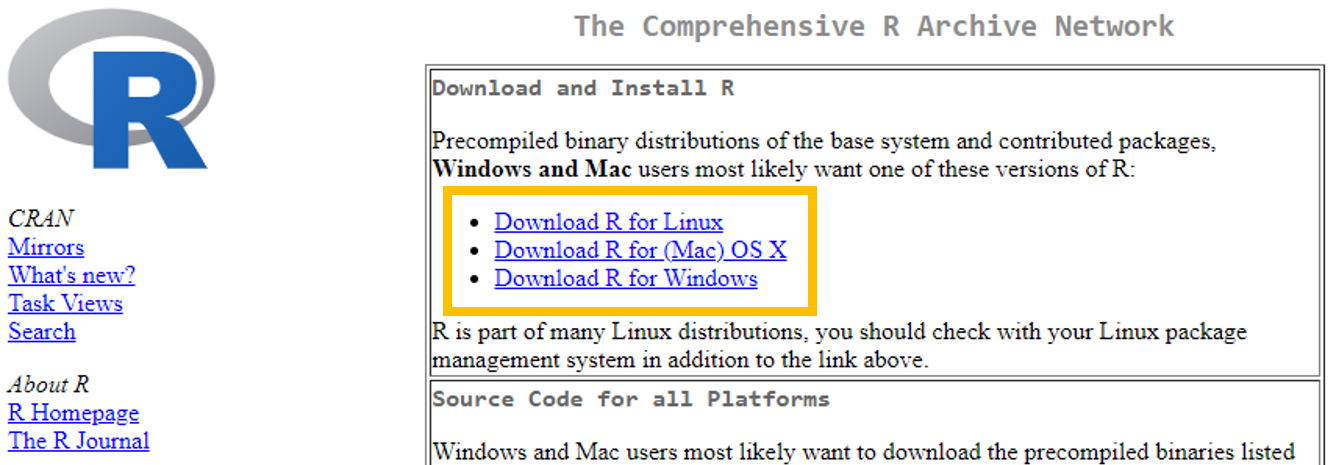
\includegraphics[keepaspectratio]{images/lab-1/r1.png}}

Next, install RStudio Desktop, which can be
\href{https://posit.co/download/rstudio-desktop/}{downloaded here} (see
screenshot below).

\pandocbounded{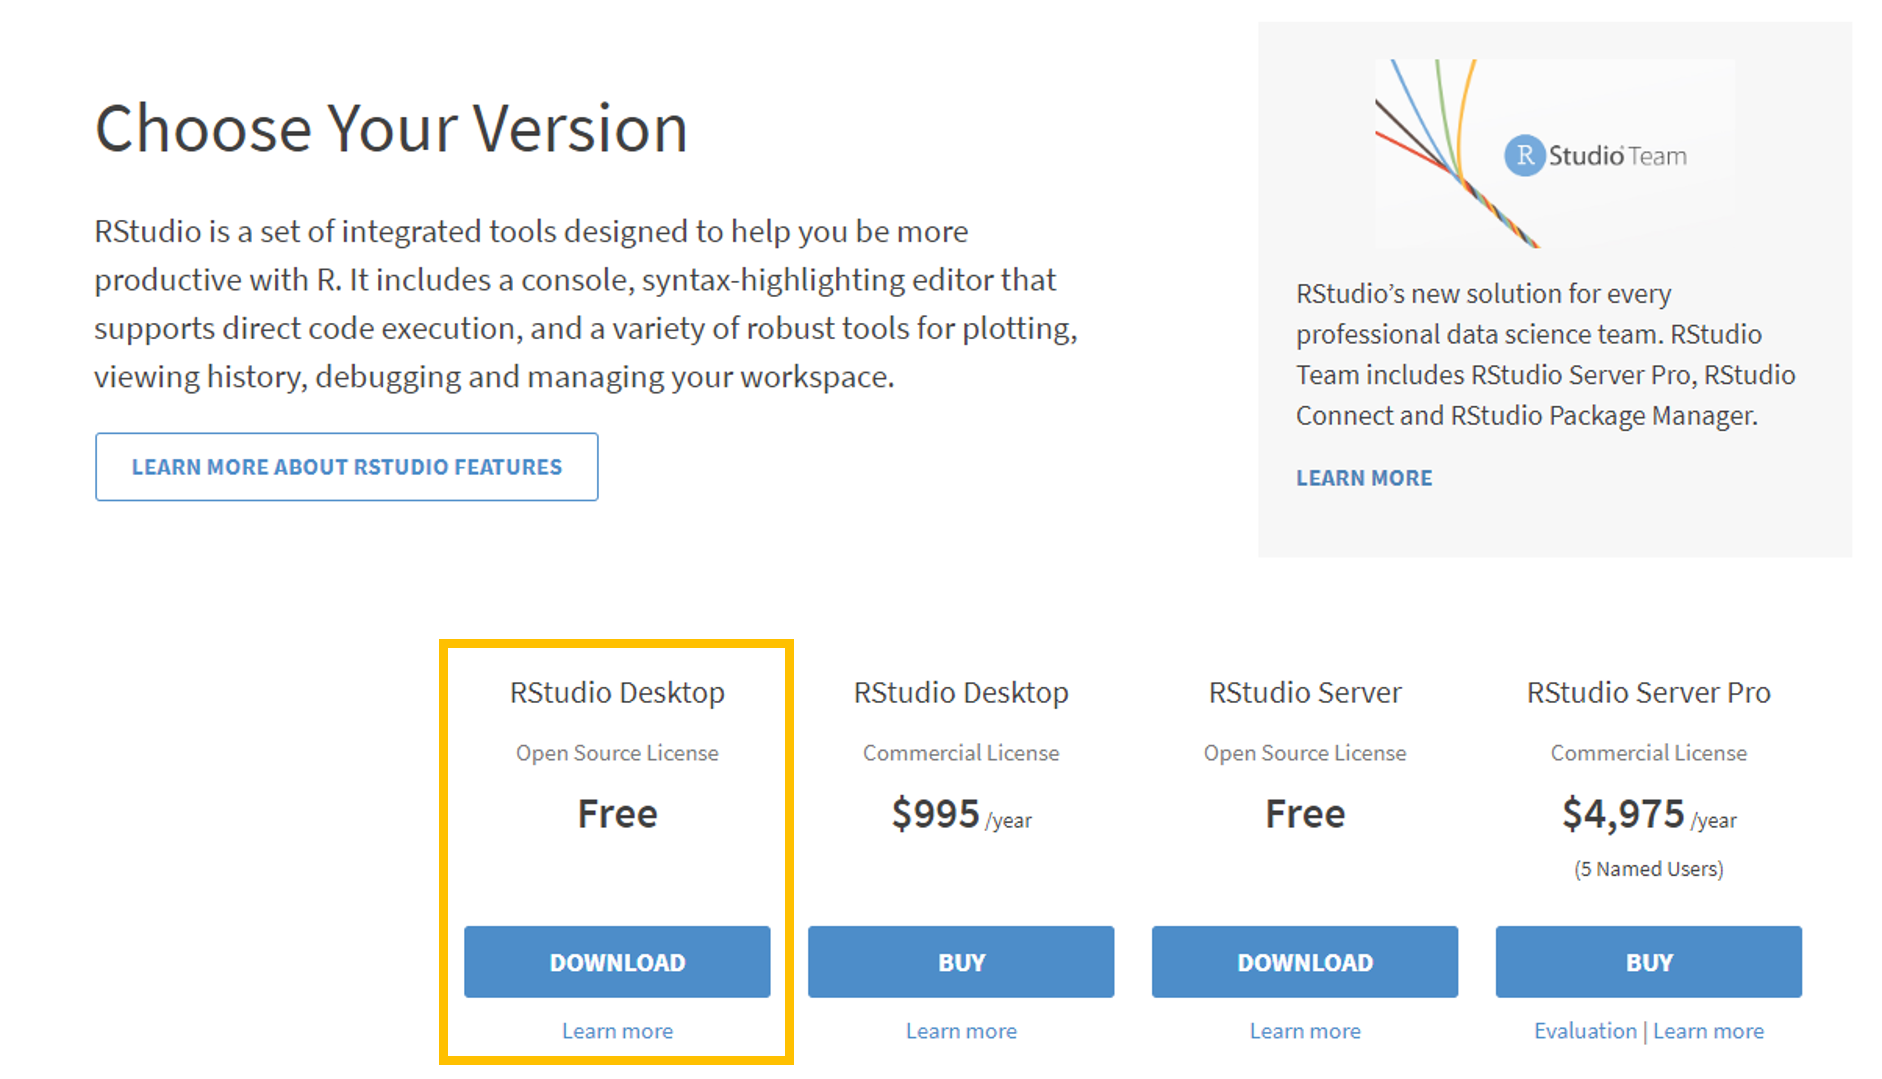
\includegraphics[keepaspectratio]{images/lab-1/r2.png}}

\subsection{First Steps in RStudio}\label{first-steps-in-rstudio}

\subsubsection{Ensure you have an updated
version}\label{ensure-you-have-an-updated-version}

For this course, we'll be using Quarto to type up HW/Labs. Quarto is a
(relatively new) publishing system which may be accessed through
RStudio. Some of you may already have R/RStudio installed on your
computer. To ensure you have a version of RStudio which can run Quarto,
follow these instructions:

\begin{itemize}
\item
  For Windows: Go to Help \textgreater{} About RStudio.
\item
  For Mac: Go to RStudio \textgreater{} About RStudio.
\item
  The dialogue box will display the RStudio version. \textbf{You should
  have version 2022.07 or later}.
\end{itemize}

\subsubsection{What if I have an earlier version of
RStudio?}\label{what-if-i-have-an-earlier-version-of-rstudio}

You'll need to update. To update RStudio, first check if an update is
available by going to Help \textgreater{} Check for Updates within
RStudio (there should be one available). If an update is found (it
should be), you'll be directed to the RStudio website to download the
latest version. After downloading, run the installer and follow the
prompts to install the new version.

\subsection{Exploring RStudio}\label{exploring-rstudio}

With R and RStudio installed, we'll begin by exploring RStudio: the
interface, reading in data, and basic commands. Upon opening RStudio,
you should see something similar to the window below:

\pandocbounded{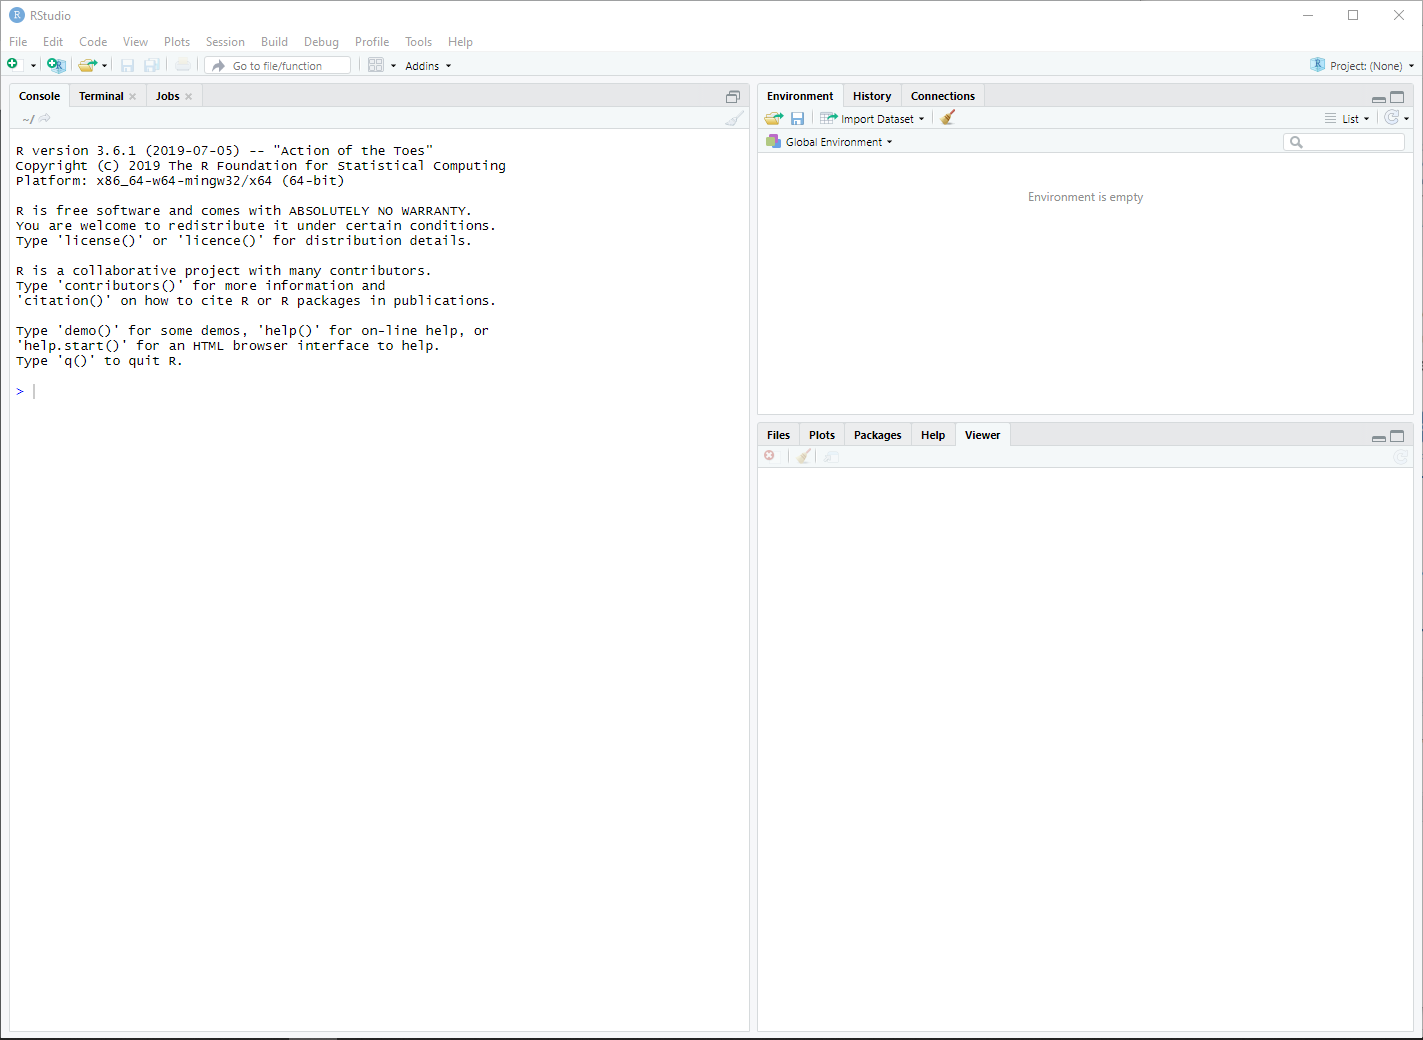
\includegraphics[keepaspectratio]{images/lab-1/r3.png}}

The \textbf{console} is the panel on the left side, and is where users
can type commands and see immediate output. Let's try it out! Type the
following code into the console:

\begin{Shaded}
\begin{Highlighting}[]
\DecValTok{3} \SpecialCharTok{+} \DecValTok{5}
\end{Highlighting}
\end{Shaded}

You should get output that looks like

\begin{verbatim}
[1] 8
\end{verbatim}

(For now, ignore the \texttt{{[}1{]}}). By typing in \texttt{3+5}, we
got the expected answer, \texttt{8}. We can see that R can be used as a
calculator directly in the console. Try some other commands that use R
as a calculator. For instance, \texttt{3*25}, \texttt{exp(2)}, or
\texttt{(10+5\^{}2)/sqrt(40)}. Of course, R is not simply a calculator;
other commands may also be entered here.

To illustrate, let's load a dataset. Enter the following command into
the console (you can directly copy/paste it, but make sure everything is
exactly as below):

\begin{Shaded}
\begin{Highlighting}[]
\NormalTok{cdc }\OtherTok{\textless{}{-}} \FunctionTok{read.csv}\NormalTok{(}\StringTok{"https://aggreenbean.github.io/Bios600/labs/data/cdc\_cleaned.csv"}\NormalTok{)}
\end{Highlighting}
\end{Shaded}

We've just loaded a dataset named \texttt{cdc}. These data come
primarily from the Sortable Risk Factors and Health Indicators dataset
from the CDC, which comprises demographic and health indices compiled
from various federal sources. This dataset is now part of our
\textbf{environment}, which is displayed on the top half and right side
of the RStudio window.

\begin{itemize}
\item
  The \textbf{environment} contains all objects in the current working
  space. These objects could be variables, lists of variables, or even
  entire datasets.
\item
  In the same location as the environment tab, the \textbf{history} tab
  displays all commands used during the current session (don't worry
  about the connections tab for now).
\item
  Finally, the bottom half of the right-hand panel shows information
  regarding files on your hard drive, installed packages, output such as
  plots, and help files or other documents.
\end{itemize}

Coming back to the dataset we loaded in, we can see that it is named
\texttt{cdc}. We can take a look at this dataset in a spreadsheet-like
window by clicking on \texttt{cdc} in the Environment tab to the right,
or by running the following code in the console:

\begin{Shaded}
\begin{Highlighting}[]
\FunctionTok{View}\NormalTok{(cdc)}
\end{Highlighting}
\end{Shaded}

Note that other objects may be added to the environment, either from
external data sources from the internet as in today's example, datasets
downloaded to your computer, or even as created as manipulations of
existing datasets.

\subsection{Setting up a project in
RStudio}\label{setting-up-a-project-in-rstudio}

In this class, you'll use RStudio Projects to stay organized. A project
keeps all of your work (scripts, data, and results) together in one
place. This is good practice for reproducible research.

\textbf{1. What is a working directory?}

\begin{itemize}
\item
  The working directory is the folder where R looks for files and saves
  results.
\item
  Think of it as R's ``current location'' on your computer.
\item
  If you try to load a dataset, R will look in your working directory
  first.
\end{itemize}

Check your current working directory by running the following in your
\textbf{Console}:

\begin{Shaded}
\begin{Highlighting}[]
\FunctionTok{getwd}\NormalTok{()}
\end{Highlighting}
\end{Shaded}

\textbf{2. Creating a project}

We'll create a new project for this course so everything stays in one
place. In RStudio, go to the top menu. Click on File → New Project → New
Directory → New Project. Name your project something sensible \&
concise, like: \texttt{bios600}. Choose where on your computer you want
this folder saved (e.g., ``Documents'' or ``Desktop'').

Now RStudio will automatically set your project folder as the working
directory whenever you open it.

\textbf{3. Creating a ``data'' folder}

Inside your new project folder, we're going to create a folder called
\texttt{data}.This is where you'll put all datasets for the course. You
can make the folder by doing the following: In your computer's file
explorer (right click → New Folder → name it \texttt{data}).
Alternatively, click the little folder with a green plus on your lower
right pane within RStudio to create the folder.

\subsection{Quarto and reproducible
research}\label{quarto-and-reproducible-research}

Quarto is a system that may be used to create easy-to-write, attractive
reports, presentations, or webpages that also serve as reproducible
records of the data analysis. These reports have the desirable property
of being able to not only display written narratives and figures, but
also include any R code and the outputs from these code snippets.

One of the biggest strengths of Quarto is that everything is in one
place, and that other users should be able to reproduce your results
exactly, if they have your Quarto document and datasets - the analysis
is run from the beginning each time you render the document. As well,
formatting is easy! Luckily, RStudio already comes with Quarto support,
so there is nothing additional to install. (Again, you need
\textgreater= version 2022.07 to run Quarto within RStudio!)

Every homework assignment and lab in this class will be written in
Quarto, with a template provided for you to use for the first few
assignments. This lab's template can be downloaded by typing in the
following code in the Console:

\begin{Shaded}
\begin{Highlighting}[]
\FunctionTok{download.file}\NormalTok{(}\StringTok{"https://github.com/mhoch422/BIOS600\_SSII/blob/main/homework/hw{-}01{-}template.qmd"}\NormalTok{, }\AttributeTok{destfile=}\StringTok{"lab{-}01.qmd"}\NormalTok{)}
\end{Highlighting}
\end{Shaded}

You should now see the new file \texttt{lab-01.qmd} under the Files tab
in the bottom-right hand side of your RStudio window. Click on
\texttt{lab-01.qmd} in this window in order to open it up -- it is the
template for use in this lab!

First, put your name in the space at the top where it says ``YOUR NAME
GOES HERE''.

Fill in answers in the spaces provided: text narrative should be typed
directly in the document and any included R code should be typed inside
``chunks,'' or sections defined by three backticks (the little mark on
the same key as the tilde). See the template for more instructions, or
ask your TA.

An important thing to note is that the workspace of the Quarto document
is separate from the console -- this means that you must load any
packages inside of R chunks if you want to use functions contained in
them. In the template for this lab, this has been done already, but in
the future you may have to do it yourself.

In order to turn this template into a shareable document,
\textbf{Render} the quarto template into an HTML document by pressing
the Render button at the top of the document (it is a large blue arrow
facing the right). You should see the template rendered as an .html
file! To turn it in, print to PDF from your browser. (I recommend Google
Chrome.)

\subsection{At the end, here's how you'll turn this
in:}\label{at-the-end-heres-how-youll-turn-this-in}

\begin{itemize}
\item
  ``Render'' the .qmd file to an html file, by clicking on the blue
  right arrow button at the top of this window. (Demo)
\item
  Open the .html document in any browser, and print to pdf. You'll turn
  in the .pdf file to Gradescope under Lab 1 Assignments.
\end{itemize}

\section{On your own}\label{on-your-own}

\subsection{Exercise 1}\label{exercise-1}

R has various useful datasets built-in. One of these datasets is the
\texttt{mtcars} dataset, extracted from the 1974 \emph{Motor Trend} US
magazine. One way we can ask for help in R, and to find out information
about the data, is by typing the \texttt{?} in the console. Type
\texttt{?mtcars} in the Console to view the help page for the
\texttt{mtcars} dataset.

List three variables from this dataset, along with their units.

\subsection{Exercise 2}\label{exercise-2}

In the space provided, explain what you think \#\#\# in front of text
(not code) does.

\subsection{Exercise 3}\label{exercise-3}

Write a quick one paragraph intro about yourself. Be creative!

\subsection{Exercise 4}\label{exercise-4}

In the R chunk, pick your two favorite numbers and add them together
using R's built-in calculator function. The answer should be knit
directly in the document.

\subsection{From .html to .pdf}\label{from-.html-to-.pdf}

Important: You must turn in a .pdf file corresponding to the Quarto
template to Gradescope in order to receive credit for the assignment.




\end{document}
